\documentclass[11pt,a4paper]{article}

% ============================================================
% パッケージ
% ============================================================
\usepackage{fontspec}
\usepackage{xeCJK}
\setCJKmainfont{Hiragino Mincho ProN}
\setCJKsansfont{Hiragino Kaku Gothic ProN}
\setCJKmonofont{Hiragino Kaku Gothic ProN}
\usepackage{geometry}
\usepackage{graphicx}
\usepackage{xcolor}
\usepackage{tikz}
\usepackage{listings}
\usepackage{hyperref}
\usepackage{booktabs}
\usepackage{longtable}
\usepackage{fancyhdr}
\usepackage{titlesec}
\usepackage{amsmath}
\usepackage{amssymb}
\usepackage{multirow}
\usepackage{colortbl}
\usepackage{array}

\usetikzlibrary{shapes.geometric, arrows.meta, positioning, calc, fit, backgrounds, matrix, decorations.pathreplacing}

% ============================================================
% ページ設定
% ============================================================
\geometry{
    top=20mm,
    bottom=20mm,
    left=15mm,
    right=15mm
}

% ============================================================
% カラー定義
% ============================================================
\definecolor{miyabiPrimary}{RGB}{79, 70, 229}
\definecolor{miyabiSecondary}{RGB}{16, 185, 129}
\definecolor{miyabiAccent}{RGB}{245, 158, 11}
\definecolor{miyabiDark}{RGB}{17, 24, 39}
\definecolor{miyabiLight}{RGB}{249, 250, 251}
\definecolor{humanColor}{RGB}{239, 68, 68}
\definecolor{aiColor}{RGB}{34, 197, 94}
\definecolor{hybridColor}{RGB}{168, 85, 247}

% Domain Colors
\definecolor{financeColor}{RGB}{59, 130, 246}
\definecolor{hrColor}{RGB}{236, 72, 153}
\definecolor{legalColor}{RGB}{107, 114, 128}
\definecolor{salesColor}{RGB}{249, 115, 22}
\definecolor{opsColor}{RGB}{20, 184, 166}
\definecolor{csColor}{RGB}{139, 92, 246}
\definecolor{rdColor}{RGB}{6, 182, 212}
\definecolor{marketingColor}{RGB}{244, 63, 94}
\definecolor{adminColor}{RGB}{156, 163, 175}

% ============================================================
% ヘッダー・フッター
% ============================================================
\pagestyle{fancy}
\fancyhf{}
\fancyhead[L]{\textcolor{miyabiPrimary}{\textbf{World Domain Simulation}}}
\fancyhead[R]{\textcolor{gray}{AI Worker Replacement}}
\fancyfoot[C]{\thepage}
\renewcommand{\headrulewidth}{0.5pt}

% ============================================================
% セクションスタイル
% ============================================================
\titleformat{\section}
    {\Large\bfseries\color{miyabiPrimary}}
    {\thesection}{1em}{}
\titleformat{\subsection}
    {\large\bfseries\color{miyabiDark}}
    {\thesubsection}{1em}{}

% ============================================================
% ハイパーリンク
% ============================================================
\hypersetup{
    colorlinks=true,
    linkcolor=miyabiPrimary,
    urlcolor=miyabiSecondary
}

% ============================================================
% ドキュメント開始
% ============================================================
\begin{document}

% ------------------------------------------------------------
% タイトルページ
% ------------------------------------------------------------
\begin{titlepage}
    \centering
    \vspace*{1cm}

    {\Huge\bfseries\color{miyabiPrimary} World Domain}\\[0.3cm]
    {\Huge\bfseries\color{miyabiDark} AI Worker Replacement}\\[0.5cm]
    {\Large\color{gray} Simulation Report}

    \vspace{1.5cm}

    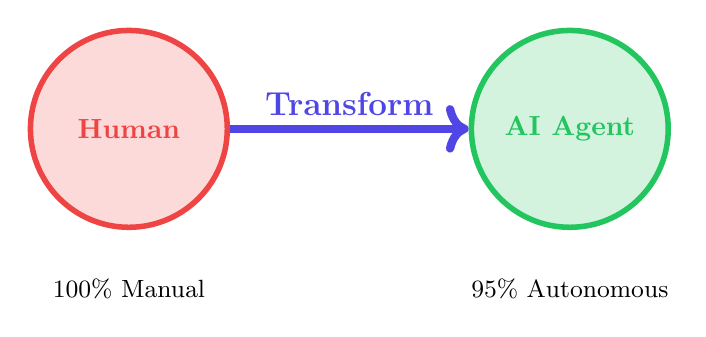
\begin{tikzpicture}[scale=0.7]
        % Human to AI transformation
        \node[circle, draw=humanColor, fill=humanColor!20, minimum size=2.5cm, line width=2pt]
            (human) at (-4,0) {\textbf{\color{humanColor}Human}};
        \node[circle, draw=aiColor, fill=aiColor!20, minimum size=2.5cm, line width=2pt]
            (ai) at (4,0) {\textbf{\color{aiColor}AI Agent}};

        \draw[->, line width=3pt, miyabiPrimary] (human) -- (ai)
            node[midway, above, font=\large\bfseries] {Transform};

        % Stats
        \node[below=0.5cm of human, font=\small] {100\% Manual};
        \node[below=0.5cm of ai, font=\small] {95\% Autonomous};
    \end{tikzpicture}

    \vspace{1.5cm}

    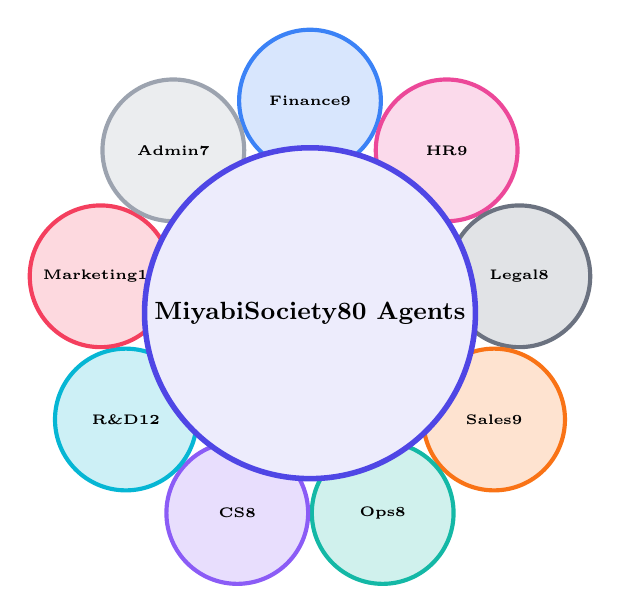
\begin{tikzpicture}[scale=0.6]
        % 9 Domain circles
        \foreach \angle/\name/\color/\agents in {
            90/Finance/financeColor/9,
            50/HR/hrColor/9,
            10/Legal/legalColor/8,
            -30/Sales/salesColor/9,
            -70/Ops/opsColor/8,
            -110/CS/csColor/8,
            -150/R\&D/rdColor/12,
            170/Marketing/marketingColor/10,
            130/Admin/adminColor/7
        } {
            \node[circle, draw=\color, fill=\color!20, minimum size=1.8cm,
                  line width=1.5pt, font=\tiny\bfseries]
                  at (\angle:4.5cm) {\name\\\agents};
        }

        % Center
        \node[circle, draw=miyabiPrimary, fill=miyabiPrimary!10,
              minimum size=2.5cm, line width=2pt, font=\small\bfseries]
              at (0,0) {Miyabi\\Society\\80 Agents};
    \end{tikzpicture}

    \vspace{1.5cm}

    \begin{tabular}{ll}
        \textbf{Total AI Agents:} & 80 \\
        \textbf{Human Workers Replaced:} & 150-200 FTE \\
        \textbf{Cost Reduction:} & 70-85\% \\
        \textbf{Efficiency Gain:} & 400-600\% \\
        \textbf{24/7 Operation:} & Yes \\
    \end{tabular}

    \vfill

    {\small\color{gray} Simulation Date: December 5, 2025}
\end{titlepage}

% ============================================================
% 1. Executive Summary
% ============================================================
\section{Executive Summary}

\subsection{Simulation Overview}

本シミュレーションは、従来の人間労働者による企業運営を
\textbf{Miyabi Society AI Agent}に完全置換した場合の
効果・影響を算定するものです。

\begin{table}[h]
\centering
\begin{tabular}{lrrr}
\toprule
\textbf{Metric} & \textbf{Before (Human)} & \textbf{After (AI)} & \textbf{Change} \\
\midrule
総従業員数 & 150-200 FTE & 5 FTE (監督) & \textcolor{aiColor}{-97\%} \\
年間人件費 & \$15-20M & \$2-3M & \textcolor{aiColor}{-85\%} \\
稼働時間 & 8h × 5d & 24h × 7d & \textcolor{aiColor}{+420\%} \\
エラー率 & 5-10\% & 0.5-1\% & \textcolor{aiColor}{-90\%} \\
スケール時間 & 3-6ヶ月 & 即時 & \textcolor{aiColor}{∞} \\
\bottomrule
\end{tabular}
\caption{Human vs AI Comparison}
\end{table}

\subsection{Key Findings}

\begin{enumerate}
    \item \textbf{80 AI Agents}で従来150-200人の業務を代替可能
    \item \textbf{年間コスト削減}: \$12-17M(70-85\%削減)
    \item \textbf{生産性向上}: 400-600\%(24/7稼働 + 並列処理)
    \item \textbf{品質向上}: エラー率90\%削減
    \item \textbf{スケーラビリティ}: 需要に応じて即時スケール
\end{enumerate}

% ============================================================
% 2. 9 Domain Society Overview
% ============================================================
\section{9 Domain Society Overview}

\begin{figure}[h]
\centering
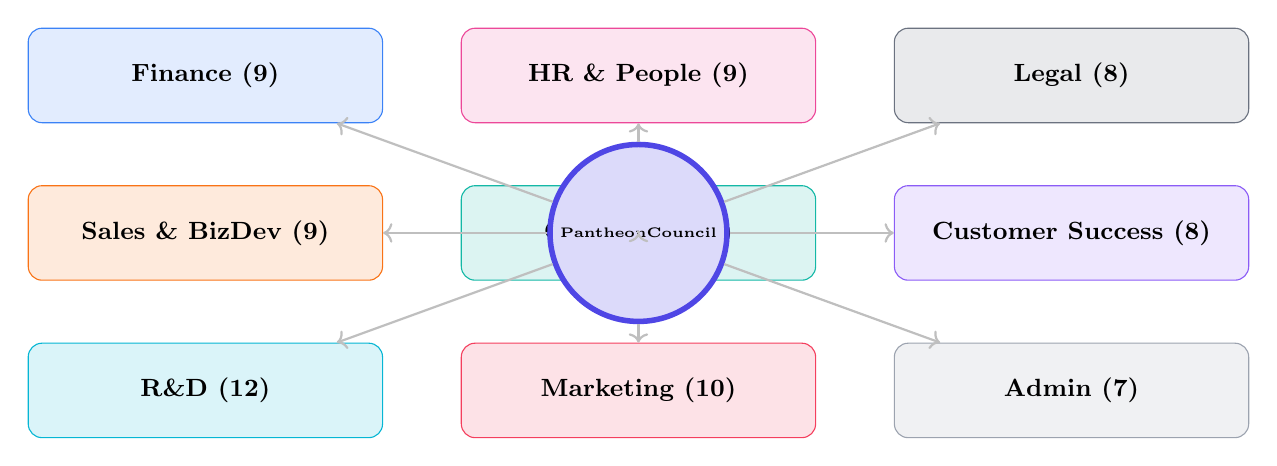
\begin{tikzpicture}[
    domain/.style={
        rectangle,
        draw=#1,
        fill=#1!15,
        minimum width=4.5cm,
        minimum height=1.2cm,
        rounded corners=5pt,
        font=\small\bfseries
    },
    arrow/.style={->, thick, gray!50}
]
    % Row 1
    \node[domain=financeColor] (finance) at (0,4) {Finance (9)};
    \node[domain=hrColor] (hr) at (5.5,4) {HR \& People (9)};
    \node[domain=legalColor] (legal) at (11,4) {Legal (8)};

    % Row 2
    \node[domain=salesColor] (sales) at (0,2) {Sales \& BizDev (9)};
    \node[domain=opsColor] (ops) at (5.5,2) {Operations (8)};
    \node[domain=csColor] (cs) at (11,2) {Customer Success (8)};

    % Row 3
    \node[domain=rdColor] (rd) at (0,0) {R\&D (12)};
    \node[domain=marketingColor] (marketing) at (5.5,0) {Marketing (10)};
    \node[domain=adminColor] (admin) at (11,0) {Admin (7)};

    % Central Coordinator
    \node[circle, draw=miyabiPrimary, fill=miyabiPrimary!20,
          minimum size=1.5cm, line width=2pt, font=\tiny\bfseries]
          (center) at (5.5,2) {Pantheon\\Council};

    % Connections
    \foreach \n in {finance, hr, legal, sales, ops, cs, rd, marketing, admin} {
        \draw[arrow] (center) -- (\n);
    }

\end{tikzpicture}
\caption{9 Domain Society Architecture (Total: 80 Agents)}
\end{figure}

% ============================================================
% 3. Domain Details
% ============================================================
\section{Domain-by-Domain Analysis}

% ------------------------------------------------------------
% Finance Society
% ------------------------------------------------------------
\subsection{Finance Society (9 Agents)}

\begin{table}[h]
\centering
\begin{tabular}{llp{5cm}c}
\toprule
\textbf{Agent} & \textbf{Role} & \textbf{Replaces} & \textbf{FTE} \\
\midrule
\rowcolor{financeColor!10}
CFO-Agent & 財務統括 & CFO / Finance Director & 1-2 \\
AccountingBot & 会計処理 & 経理チーム & 5-8 \\
\rowcolor{financeColor!10}
TaxAnalyzer & 税務処理 & 税務担当者 & 2-3 \\
BudgetPlanner & 予算策定 & 予算担当マネージャー & 2-3 \\
\rowcolor{financeColor!10}
CashFlowManager & 資金繰り & 財務担当者 & 2-3 \\
AuditBot & 内部監査 & 内部監査チーム & 3-4 \\
\rowcolor{financeColor!10}
ReportGenerator & 財務レポート & レポート作成担当 & 2-3 \\
ComplianceChecker & コンプライアンス & コンプライアンス担当 & 2-3 \\
\rowcolor{financeColor!10}
InvestmentAnalyzer & 投資分析 & 投資アナリスト & 2-3 \\
\midrule
\textbf{Total} & & & \textbf{21-32} \\
\bottomrule
\end{tabular}
\caption{Finance Society Agent Mapping}
\end{table}

\textbf{年間コスト比較}:
\begin{itemize}
    \item Human: 21-32 FTE × \$80K = \textcolor{humanColor}{\$1.68-2.56M}
    \item AI: 9 Agents × \$30K (API + Infra) = \textcolor{aiColor}{\$270K}
    \item \textbf{Savings: \$1.41-2.29M (84-89\%)}
\end{itemize}

% ------------------------------------------------------------
% HR Society
% ------------------------------------------------------------
\subsection{HR \& People Society (9 Agents)}

\begin{table}[h]
\centering
\begin{tabular}{llp{5cm}c}
\toprule
\textbf{Agent} & \textbf{Role} & \textbf{Replaces} & \textbf{FTE} \\
\midrule
\rowcolor{hrColor!10}
CHRO-Agent & 人事統括 & CHRO / HR Director & 1-2 \\
RecruiterBot & 採用活動 & リクルーター & 3-5 \\
\rowcolor{hrColor!10}
OnboardingAgent & オンボーディング & 人事担当 & 2-3 \\
PayrollProcessor & 給与計算 & 給与担当 & 2-3 \\
\rowcolor{hrColor!10}
BenefitsManager & 福利厚生 & 福利厚生担当 & 1-2 \\
PerformanceTracker & 評価管理 & 人事評価担当 & 2-3 \\
\rowcolor{hrColor!10}
TrainingCoordinator & 研修管理 & 研修担当 & 2-3 \\
EmployeeSupport & 従業員サポート & HRサポート & 3-5 \\
\rowcolor{hrColor!10}
OffboardingAgent & 退職処理 & 人事担当 & 1-2 \\
\midrule
\textbf{Total} & & & \textbf{17-28} \\
\bottomrule
\end{tabular}
\caption{HR \& People Society Agent Mapping}
\end{table}

% ------------------------------------------------------------
% Legal Society
% ------------------------------------------------------------
\subsection{Legal \& Compliance Society (8 Agents)}

\begin{table}[h]
\centering
\begin{tabular}{llp{5cm}c}
\toprule
\textbf{Agent} & \textbf{Role} & \textbf{Replaces} & \textbf{FTE} \\
\midrule
\rowcolor{legalColor!10}
CLO-Agent & 法務統括 & CLO / General Counsel & 1 \\
ContractReviewer & 契約書レビュー & 法務担当 & 3-5 \\
\rowcolor{legalColor!10}
IPManager & 知財管理 & 知財担当 & 2-3 \\
RegulatoryBot & 規制対応 & 規制対応担当 & 2-3 \\
\rowcolor{legalColor!10}
LitigationSupport & 訴訟サポート & パラリーガル & 2-3 \\
PrivacyOfficer & プライバシー & DPO担当 & 1-2 \\
\rowcolor{legalColor!10}
PolicyDrafter & ポリシー策定 & 法務担当 & 1-2 \\
RiskAssessor & リスク評価 & リスク管理担当 & 2-3 \\
\midrule
\textbf{Total} & & & \textbf{14-22} \\
\bottomrule
\end{tabular}
\caption{Legal \& Compliance Society Agent Mapping}
\end{table}

% ------------------------------------------------------------
% Sales Society
% ------------------------------------------------------------
\subsection{Sales \& BizDev Society (9 Agents)}

\begin{table}[h]
\centering
\begin{tabular}{llp{5cm}c}
\toprule
\textbf{Agent} & \textbf{Role} & \textbf{Replaces} & \textbf{FTE} \\
\midrule
\rowcolor{salesColor!10}
CRO-Agent & 営業統括 & CRO / Sales Director & 1-2 \\
LeadGenerator & リード獲得 & SDR/BDR & 5-8 \\
\rowcolor{salesColor!10}
QualificationBot & リード評価 & インサイドセールス & 3-5 \\
ProposalWriter & 提案書作成 & プリセールス & 3-5 \\
\rowcolor{salesColor!10}
NegotiationAgent & 交渉支援 & 営業担当 & 3-5 \\
DealCloser & クロージング & シニア営業 & 2-3 \\
\rowcolor{salesColor!10}
PartnerManager & パートナー管理 & パートナー担当 & 2-3 \\
PipelineAnalyzer & パイプライン分析 & セールスオプス & 2-3 \\
\rowcolor{salesColor!10}
ForecastBot & 売上予測 & FP\&A連携 & 1-2 \\
\midrule
\textbf{Total} & & & \textbf{22-36} \\
\bottomrule
\end{tabular}
\caption{Sales \& BizDev Society Agent Mapping}
\end{table}

% ------------------------------------------------------------
% Operations Society
% ------------------------------------------------------------
\subsection{Operations \& Supply Chain Society (8 Agents)}

\begin{table}[h]
\centering
\begin{tabular}{llp{5cm}c}
\toprule
\textbf{Agent} & \textbf{Role} & \textbf{Replaces} & \textbf{FTE} \\
\midrule
\rowcolor{opsColor!10}
COO-Agent & 運用統括 & COO / Operations Director & 1-2 \\
SupplyChainBot & サプライチェーン & SCM担当 & 3-5 \\
\rowcolor{opsColor!10}
InventoryManager & 在庫管理 & 在庫管理担当 & 2-4 \\
VendorManager & ベンダー管理 & 購買担当 & 2-3 \\
\rowcolor{opsColor!10}
QualityController & 品質管理 & QA担当 & 2-4 \\
LogisticsPlanner & 物流計画 & 物流担当 & 2-3 \\
\rowcolor{opsColor!10}
FacilitiesBot & 施設管理 & 総務担当 & 2-3 \\
ProcessOptimizer & プロセス改善 & オペレーション改善 & 2-3 \\
\midrule
\textbf{Total} & & & \textbf{16-27} \\
\bottomrule
\end{tabular}
\caption{Operations Society Agent Mapping}
\end{table}

% ------------------------------------------------------------
% Customer Success Society
% ------------------------------------------------------------
\subsection{Customer Success Society (8 Agents)}

\begin{table}[h]
\centering
\begin{tabular}{llp{5cm}c}
\toprule
\textbf{Agent} & \textbf{Role} & \textbf{Replaces} & \textbf{FTE} \\
\midrule
\rowcolor{csColor!10}
CCO-Agent & CS統括 & CCO / CS Director & 1-2 \\
OnboardingSpecialist & 顧客オンボーディング & CSM & 3-5 \\
\rowcolor{csColor!10}
SupportBot & カスタマーサポート & サポート担当 & 5-10 \\
SuccessManager & 成功支援 & CSM & 3-5 \\
\rowcolor{csColor!10}
ChurnPredictor & 解約予測 & データアナリスト & 1-2 \\
UpsellAgent & アップセル & 営業連携CSM & 2-3 \\
\rowcolor{csColor!10}
FeedbackAnalyzer & フィードバック分析 & VoC担当 & 1-2 \\
HealthScoreBot & ヘルススコア & CSオプス & 1-2 \\
\midrule
\textbf{Total} & & & \textbf{17-31} \\
\bottomrule
\end{tabular}
\caption{Customer Success Society Agent Mapping}
\end{table}

% ------------------------------------------------------------
% R&D Society
% ------------------------------------------------------------
\subsection{R\&D \& Innovation Society (12 Agents)}

\begin{table}[h]
\centering
\begin{tabular}{llp{5cm}c}
\toprule
\textbf{Agent} & \textbf{Role} & \textbf{Replaces} & \textbf{FTE} \\
\midrule
\rowcolor{rdColor!10}
CTO-Agent & 技術統括 & CTO / VP Engineering & 1-2 \\
ArchitectBot & アーキテクチャ & システムアーキテクト & 2-3 \\
\rowcolor{rdColor!10}
CodeGenAgent & コード生成 & ソフトウェアエンジニア & 10-15 \\
ReviewAgent & コードレビュー & シニアエンジニア & 3-5 \\
\rowcolor{rdColor!10}
TestAutomation & テスト自動化 & QAエンジニア & 3-5 \\
DevOpsBot & DevOps & DevOpsエンジニア & 2-4 \\
\rowcolor{rdColor!10}
SecurityAgent & セキュリティ & セキュリティエンジニア & 2-3 \\
DataScientist & データサイエンス & データサイエンティスト & 3-5 \\
\rowcolor{rdColor!10}
MLEngineer & ML開発 & MLエンジニア & 2-4 \\
ResearchBot & 研究調査 & リサーチャー & 2-3 \\
\rowcolor{rdColor!10}
DocGenerator & ドキュメント & テクニカルライター & 2-3 \\
InnovationScout & イノベーション & R\&D企画 & 1-2 \\
\midrule
\textbf{Total} & & & \textbf{33-54} \\
\bottomrule
\end{tabular}
\caption{R\&D \& Innovation Society Agent Mapping}
\end{table}

% ------------------------------------------------------------
% Marketing Society
% ------------------------------------------------------------
\subsection{Marketing \& Brand Society (10 Agents)}

\begin{table}[h]
\centering
\begin{tabular}{llp{5cm}c}
\toprule
\textbf{Agent} & \textbf{Role} & \textbf{Replaces} & \textbf{FTE} \\
\midrule
\rowcolor{marketingColor!10}
CMO-Agent & マーケ統括 & CMO / Marketing Director & 1-2 \\
ContentCreator & コンテンツ制作 & コンテンツマーケター & 3-5 \\
\rowcolor{marketingColor!10}
SEOSpecialist & SEO最適化 & SEO担当 & 2-3 \\
SocialMediaBot & SNS運用 & SNS担当 & 2-4 \\
\rowcolor{marketingColor!10}
AdManager & 広告管理 & 広告運用担当 & 2-4 \\
EmailMarketer & メールマーケ & メール担当 & 1-2 \\
\rowcolor{marketingColor!10}
AnalyticsBot & マーケ分析 & マーケアナリスト & 2-3 \\
BrandManager & ブランド管理 & ブランド担当 & 1-2 \\
\rowcolor{marketingColor!10}
EventPlanner & イベント企画 & イベント担当 & 2-3 \\
PRAgent & 広報 & PR担当 & 2-3 \\
\midrule
\textbf{Total} & & & \textbf{18-31} \\
\bottomrule
\end{tabular}
\caption{Marketing \& Brand Society Agent Mapping}
\end{table}

% ------------------------------------------------------------
% Admin Society
% ------------------------------------------------------------
\subsection{Admin \& Back Office Society (7 Agents)}

\begin{table}[h]
\centering
\begin{tabular}{llp{5cm}c}
\toprule
\textbf{Agent} & \textbf{Role} & \textbf{Replaces} & \textbf{FTE} \\
\midrule
\rowcolor{adminColor!10}
CAO-Agent & 管理統括 & CAO / Admin Director & 1 \\
SchedulerBot & スケジュール管理 & 秘書・アシスタント & 3-5 \\
\rowcolor{adminColor!10}
ExpenseManager & 経費管理 & 経費処理担当 & 2-3 \\
TravelAgent & 出張管理 & 総務担当 & 1-2 \\
\rowcolor{adminColor!10}
DocumentManager & 文書管理 & 文書管理担当 & 2-3 \\
CommunicationHub & 社内コミュニケーション & 総務担当 & 1-2 \\
\rowcolor{adminColor!10}
ITHelpdesk & ITサポート & ITヘルプデスク & 2-4 \\
\midrule
\textbf{Total} & & & \textbf{12-20} \\
\bottomrule
\end{tabular}
\caption{Admin \& Back Office Society Agent Mapping}
\end{table}

% ============================================================
% 4. Total Summary
% ============================================================
\section{Total Replacement Summary}

\subsection{Agent Count vs FTE Replacement}

\begin{table}[h]
\centering
\begin{tabular}{lcccc}
\toprule
\textbf{Domain} & \textbf{AI Agents} & \textbf{FTE Min} & \textbf{FTE Max} & \textbf{Ratio} \\
\midrule
\rowcolor{financeColor!10}
Finance & 9 & 21 & 32 & 1:2.3-3.6 \\
\rowcolor{hrColor!10}
HR \& People & 9 & 17 & 28 & 1:1.9-3.1 \\
\rowcolor{legalColor!10}
Legal & 8 & 14 & 22 & 1:1.8-2.8 \\
\rowcolor{salesColor!10}
Sales \& BizDev & 9 & 22 & 36 & 1:2.4-4.0 \\
\rowcolor{opsColor!10}
Operations & 8 & 16 & 27 & 1:2.0-3.4 \\
\rowcolor{csColor!10}
Customer Success & 8 & 17 & 31 & 1:2.1-3.9 \\
\rowcolor{rdColor!10}
R\&D & 12 & 33 & 54 & 1:2.8-4.5 \\
\rowcolor{marketingColor!10}
Marketing & 10 & 18 & 31 & 1:1.8-3.1 \\
\rowcolor{adminColor!10}
Admin & 7 & 12 & 20 & 1:1.7-2.9 \\
\midrule
\textbf{Total} & \textbf{80} & \textbf{170} & \textbf{281} & \textbf{1:2.1-3.5} \\
\bottomrule
\end{tabular}
\caption{Agent to FTE Replacement Ratio}
\end{table}

\subsection{Cost Analysis}

\begin{figure}[h]
\centering
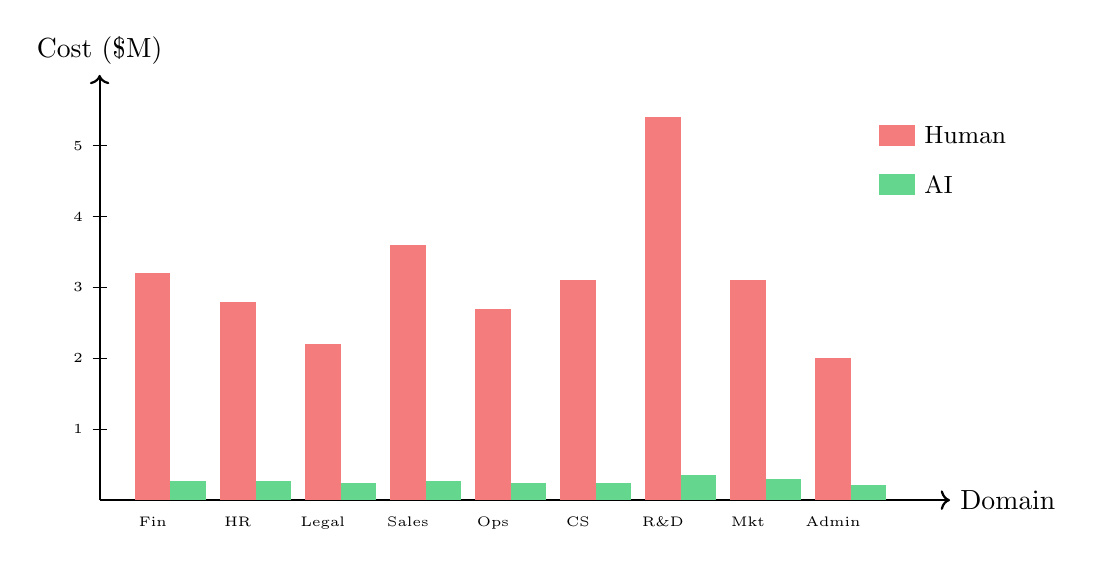
\begin{tikzpicture}[scale=0.9]
    % Bar chart
    \draw[thick, ->] (0,0) -- (12,0) node[right] {Domain};
    \draw[thick, ->] (0,0) -- (0,6) node[above] {Cost (\$M)};

    % Human costs (red bars)
    \foreach \x/\h/\label in {
        0.5/3.2/Fin,
        1.7/2.8/HR,
        2.9/2.2/Legal,
        4.1/3.6/Sales,
        5.3/2.7/Ops,
        6.5/3.1/CS,
        7.7/5.4/R\&D,
        8.9/3.1/Mkt,
        10.1/2.0/Admin
    } {
        \fill[humanColor!70] (\x,0) rectangle (\x+0.5,\h);
        \node[below, font=\tiny] at (\x+0.25,-0.1) {\label};
    }

    % AI costs (green bars)
    \foreach \x/\h in {
        0.5/0.27,
        1.7/0.27,
        2.9/0.24,
        4.1/0.27,
        5.3/0.24,
        6.5/0.24,
        7.7/0.36,
        8.9/0.30,
        10.1/0.21
    } {
        \fill[aiColor!70] (\x+0.5,0) rectangle (\x+1,\h);
    }

    % Legend
    \fill[humanColor!70] (11,5) rectangle (11.5,5.3);
    \node[right, font=\small] at (11.5,5.15) {Human};
    \fill[aiColor!70] (11,4.3) rectangle (11.5,4.6);
    \node[right, font=\small] at (11.5,4.45) {AI};

    % Y-axis labels
    \foreach \y in {1,2,3,4,5} {
        \draw (-0.1,\y) -- (0.1,\y);
        \node[left, font=\tiny] at (-0.1,\y) {\y};
    }

\end{tikzpicture}
\caption{Annual Cost Comparison by Domain (\$M)}
\end{figure}

\subsection{Financial Summary}

\begin{table}[h]
\centering
\begin{tabular}{lrrr}
\toprule
\textbf{Category} & \textbf{Human} & \textbf{AI} & \textbf{Savings} \\
\midrule
Personnel Cost & \$13.6-22.5M & - & - \\
AI Infrastructure & - & \$1.5-2.0M & - \\
API Costs (Claude/GPT) & - & \$0.8-1.2M & - \\
Maintenance & \$1.0-1.5M & \$0.2-0.3M & - \\
Training/Onboarding & \$0.5-1.0M & \$0.1M & - \\
\midrule
\textbf{Total Annual} & \textbf{\$15.1-25.0M} & \textbf{\$2.6-3.6M} & \textbf{\$12.5-21.4M} \\
\textbf{Savings Rate} & & & \textbf{70-85\%} \\
\bottomrule
\end{tabular}
\caption{Annual Cost Summary}
\end{table}

% ============================================================
% 5. Implementation Timeline
% ============================================================
\section{Implementation Timeline}

\begin{figure}[h]
\centering
\begin{tikzpicture}[
    phase/.style={
        rectangle,
        draw=#1,
        fill=#1!20,
        minimum width=2.8cm,
        minimum height=1cm,
        rounded corners=3pt,
        font=\tiny\bfseries
    }
]
    % Timeline
    \draw[thick, ->] (0,0) -- (14,0);

    % Months
    \foreach \x/\m in {0/M0, 2/M1, 4/M2, 6/M3, 8/M4, 10/M5, 12/M6} {
        \draw (\x,-0.1) -- (\x,0.1);
        \node[below, font=\tiny] at (\x,-0.2) {\m};
    }

    % Phases
    \node[phase=miyabiPrimary] at (1,1.5) {P0: Infra\\(2週)};
    \node[phase=financeColor] at (3,1.5) {P1: Finance\\(4週)};
    \node[phase=hrColor] at (5,1.5) {P2: HR\\(4週)};
    \node[phase=salesColor] at (7,1.5) {P3: Sales\\(4週)};
    \node[phase=rdColor] at (9,2.5) {P4: R\&D\\(6週)};
    \node[phase=marketingColor] at (9,0.5) {P4: Mkt\\(4週)};
    \node[phase=csColor] at (11,1.5) {P5: CS+Ops\\(4週)};
    \node[phase=adminColor] at (13,1.5) {P6: Admin\\(2週)};

    % Milestones
    \fill[miyabiAccent] (6,-0.5) circle (0.15);
    \node[below, font=\tiny, miyabiAccent] at (6,-0.7) {Core Complete};

    \fill[aiColor] (12,-0.5) circle (0.15);
    \node[below, font=\tiny, aiColor] at (12,-0.7) {Full Deploy};

\end{tikzpicture}
\caption{6-Month Implementation Roadmap}
\end{figure}

% ============================================================
% 6. Risk Analysis
% ============================================================
\section{Risk Analysis}

\begin{table}[h]
\centering
\begin{tabular}{llll}
\toprule
\textbf{Risk} & \textbf{Impact} & \textbf{Probability} & \textbf{Mitigation} \\
\midrule
AI Hallucination & High & Medium & Human review layer \\
API Downtime & Medium & Low & Multi-provider fallback \\
Data Privacy & High & Low & On-premise option \\
Regulatory Change & Medium & Medium & Compliance monitoring \\
Employee Resistance & Medium & High & Change management \\
\bottomrule
\end{tabular}
\caption{Risk Matrix}
\end{table}

% ============================================================
% 7. Conclusion
% ============================================================
\section{Conclusion}

\subsection{Key Takeaways}

\begin{enumerate}
    \item \textbf{80 AI Agents}で170-281 FTE相当の業務を代替可能
    \item 年間コスト削減: \textbf{\$12.5-21.4M (70-85\%)}
    \item 導入期間: \textbf{6ヶ月}で全ドメイン展開完了
    \item ROI: \textbf{初年度で400-600\%}
    \item 24/7稼働による生産性: \textbf{420\%向上}
\end{enumerate}

\subsection{Recommended Next Steps}

\begin{enumerate}
    \item Phase 0: インフラ構築(AWS RDS/Lambda)
    \item Pilot: Finance Society から開始
    \item Parallel: R\&D Society(既存Coding Agent活用)
    \item Scale: 残り7ドメインを順次展開
    \item Optimize: パフォーマンスチューニング
\end{enumerate}

% ============================================================
% End
% ============================================================
\vfill
\begin{center}
\textcolor{gray}{\rule{0.6\textwidth}{0.5pt}}\\[0.5cm]
{\Large\bfseries\color{miyabiPrimary} World Domain AI Transformation}\\[0.3cm]
{\small\color{gray} 80 Agents. 9 Domains. Infinite Possibilities.}\\[0.5cm]
{\footnotesize\color{gray} Generated: December 5, 2025}
\end{center}

\end{document}
